\documentclass[11pt,aspectratio=169,handout]{beamer}

\usetheme{Singapore}
\usecolortheme{orchid}

\usepackage[utf8]{inputenc}
\usepackage[russian]{babel}
\usepackage{amsmath}
\usepackage{amsfonts}
\usepackage{amssymb}
\usepackage{graphicx}
\usepackage{bibentry}
\usepackage{wasysym}
\usepackage[most]{tcolorbox}
\usepackage[normalem]{ulem}

\usepackage{hyperref}

\definecolor{info}{RGB}{62, 180, 137}
\definecolor{warn}{RGB}{128, 0, 0}

\author{Петр Погорелов\\Олег Сапрыкин}
\title{Классические алгоритмы рекомендаций}

\logo{\includegraphics[width=.05\textwidth]{images/ok_logo.png}}

\AtBeginSection[]{
  \begin{frame}
  \vfill
  \centering
  \begin{beamercolorbox}[sep=8pt,center,shadow=true,rounded=true]{title}
    \usebeamerfont{title}\insertsectionhead\par
  \end{beamercolorbox}
  \vfill
  \end{frame}
}

\begin{document}

{
\setbeamertemplate{headline}{}

\begin{frame}
\titlepage
\end{frame}

%\begin{frame}
%\tableofcontents
%\end{frame}

}

\begin{frame}{Контекст}

\begin{center}
\includegraphics[scale=0.23]{images/mendeley.jpeg}
\end{center}

\end{frame}

\begin{frame}

\begin{columns}

\begin{column}{0.47\textwidth} 

\begin{center}
\includegraphics[scale=0.22]{images/taxonomy.png}
\end{center}

\end{column}

\begin{column}{0.47\textwidth} 

\begin{center}
\includegraphics[scale=0.2]{images/karlson.png}
\end{center}

\end{column}

\end{columns}

\end{frame}

\section{Model-based Collaborative Filtering}

\begin{frame}{Model-based CF}

\begin{tcolorbox}[colback=info!5,colframe=info!80,title=Идея]
Выучим модель, которая поможет заполнить ``пробелы'' в user-item матрице.
\end{tcolorbox}

\begin{center}
\includegraphics[scale=0.5]{images/utility-2.png}
\end{center}

\[
\hat r_{ui} = f(u, i)
\]

\end{frame}

\begin{frame}{Бейзлайн \cite{KOREN}}

\begin{columns}
\begin{column}{0.2\textwidth} 
\end{column}
\begin{column}{0.5\textwidth} 
\begin{tcolorbox}[colback=info!5,colframe=info!80,title=Модель]
\[
b_{ui} = \mu + b_u + b_i
\]
\end{tcolorbox}
\end{column}
\begin{column}{0.2\textwidth} 
\end{column}
\end{columns}

\vfill

\begin{itemize}
\item $\mu$ -- средний рейтинг
\item $b_u$ -- bias пользователя
\item $b_i$ -- bias айтема
\end{itemize}

\vfill

Оптимизируем
\[
\sum_{u, i} (b_{ui} - \mu - b_u - b_i)^2 + \lambda_1 b_u^2 + \lambda_2 b_i^2 \rightarrow min_{b_u, b_i}
\]
\begin{itemize}
\item $\lambda_1$, $\lambda_2$ -- параметры регуляризации
\end{itemize}

\end{frame}

\begin{frame}{Сингулярное разложение (SVD)}

\begin{columns}
\begin{column}{0.2\textwidth} 
\end{column}
\begin{column}{0.5\textwidth} 
\begin{tcolorbox}[colback=info!5,colframe=info!80,title=Модель]
\[
\hat r_{ui} = \mu + b_u + b_i + q_i^T p_u
\]
\end{tcolorbox}
\end{column}
\begin{column}{0.2\textwidth} 
\end{column}
\end{columns}

\vfill

\begin{itemize}
\item $q_i$ -- латентное представление айтема
\item $p_u$ -- латентное представление пользователя
\end{itemize}

\vfill

Оптимизируем
\[
\sum_{u, i} (r_{ui} - \mu - b_u - b_i - q_i^T p_u)^2 + \lambda (b_u^2 +  b_i^2 + \| q_i \|^2 + \| p_u \|^2) \rightarrow min_{b_u, b_i, p_u, q_i}
\]

\end{frame}

\begin{frame}
\begin{center}
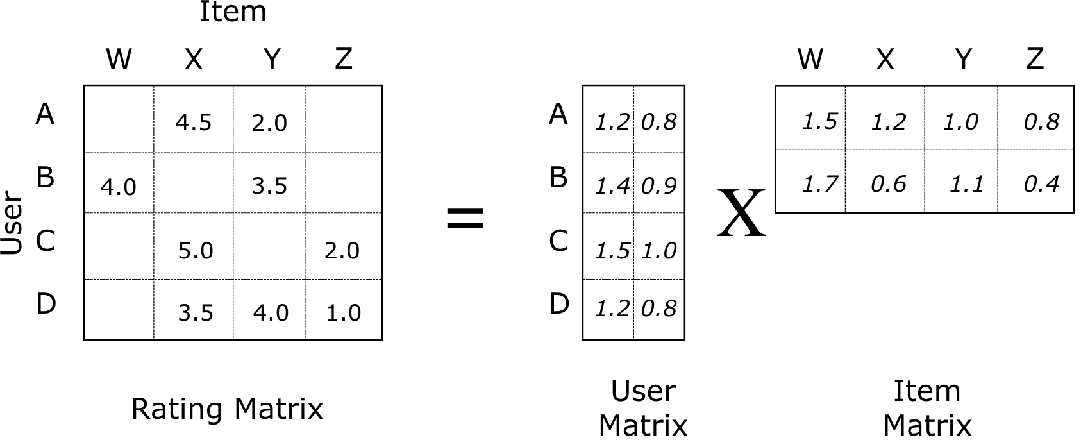
\includegraphics[scale=0.5]{images/SVD.png}
\end{center}
\end{frame}

\begin{frame}
\begin{center}
\includegraphics[scale=0.3]{images/latent.png}
\end{center}
\end{frame}

\begin{frame}{Как оптимизировать}
\[
\sum_{u, i} (r_{ui} - \mu - b_u - b_i - q_i^T p_u)^2 + \lambda (b_u^2 +  b_i^2 + \| q_i \|^2 + \| p_u \|^2)
\]

\begin{itemize}
\item ALS \cite{IMPLICIT}
% Линейное врем по N!
\begin{enumerate}
\item фиксируем $p_u, b_u$, оптимизируем $q_i, b_i$ -- получем линрег 1
\item фиксируем  $q_i, b_i$, оптимизируем $p_u, b_u$ -- получем линрег 2
\item повторяем до сходимости
\end{enumerate}
\item SGD
\[
e_{ui} = r_{ui} - \mu - b_u - b_i - q_i^T p_u 
\]
\[
b_u = b_u + \gamma * (e_{ui} - \lambda * b_u) 
\]
\[
b_i = b_i + \gamma * (e_{ui} - \lambda * b_i) 
\]
\[
q_i = q_i + \gamma * (e_{ui}*p_u - \lambda * q_i) 
\]
\[
p_i = p_i + \gamma * (e_{ui}*q_i - \lambda * p_u)
\]
\end{itemize}

\end{frame}

\begin{frame}{SVD++}

\begin{columns}
\begin{column}{0.1\textwidth} 
\end{column}
\begin{column}{0.7\textwidth} 
\begin{tcolorbox}[colback=info!5,colframe=info!80,title=Модель]
\[
\hat r_{ui} = \mu + b_u + b_i + q_i^T \left( p_u + \frac{1}{\sqrt{|R(u)|}} \sum_j y_j \right)
\]
\end{tcolorbox}
\end{column}
\begin{column}{0.1\textwidth} 
\end{column}
\end{columns}

\vfill

\begin{itemize}
\item $y_i$ -- латентное представление айтемов, на которые пользователь дал implicit feedback до оценки айтема $i$
\end{itemize}

\end{frame}

\begin{frame}{Time SVD++}

\begin{tcolorbox}[colback=info!5,colframe=info!80,title=Модель]
\[
\hat r_{ui} = \mu + b_u(t_{ui}) + b_i(t_{ui}) + q_i^T \left( p_u(t_{ui}) + \frac{1}{\sqrt{|R(u)|}} \sum_j y_j \right)
\]
\end{tcolorbox}

\vfill

\begin{itemize}
\item $t_{ui}$ -- время, когда пользователь оценил айтем
\end{itemize}

\end{frame}

\begin{frame}{Netflix Prize }

\begin{center}
\includegraphics[scale=0.25]{images/svd-compare.png}
\end{center}

\begin{small}
September 21, 2009, the grand prize of US\$1,000,000 was given to the BellKor's Pragmatic Chaos team which bested Netflix's own algorithm for predicting ratings by 10.06
\end{small}

\end{frame}

\begin{frame}{LightFM \cite{LIGHT}}

\begin{tcolorbox}[colback=info!5,colframe=info!80,title=Модель]
\[
\hat r_{ui} = \mu + b_u + b_i + q_i^T p_u
\]
\[
q_i = \sum_{j \in f_i} v_j, \quad p_u = \sum_{j \in f_u} w_j
\]
\end{tcolorbox}

\vfill

\begin{itemize}
\item $f_i$ -- признаки айтема
\item $v_j$ -- латентное представление признаков айтема
\item $f_u$ -- признаки пользователя
\item $w_j$ -- латентное представление признаков пользователя
\end{itemize}

\end{frame}

\begin{frame}{Альтернативные loss-функции: classification vs regression}

\begin{tcolorbox}[colback=info!5,colframe=info!80,title=]
Случай implicit feedback похож скорее на задачу классификации, чем регресии
\end{tcolorbox}

\[
\hat p_{ui}(r=1) = \sigma(\mu + b_u + b_i + q_i^T p_u)
\]

Лосс: кросс-энтропия

\end{frame}

\begin{frame}{Альтернативные loss-функции: ranking with BPR \cite{BPR}}

\begin{tcolorbox}[colback=info!5,colframe=info!80,title=]
Правильное ранжирование важнее, чем точное предсказание рейтинга / фидбэка
\end{tcolorbox}

\[
\hat p(u \, prefers \, i \, to \, j) = \sigma(\hat x_{uij}) = \sigma(\hat x_{ui} - \hat x_{uj})
\]
Лосс:
\[
- \sum \log p(u \, prefers \, i \, to \, j) + \lambda \| \theta \|^2
\]

\end{frame}

\begin{frame}{Альтернативные loss-функции: WARP \cite{WARP}}

\begin{tcolorbox}[colback=info!5,colframe=info!80,title=]
Можно умно семплировать негативные примеры -- так, чтобы сложность негативных примеров увеличивалась, когда модель становится точнее.
\end{tcolorbox}

Дано: пользователь + позитивный айтем
\begin{enumerate}
\item Семплируем негативные, пока не найдем неправильно отранжированную пару. Делаем шаг обновления.
\item Чем больше пришлось семплировать, тем меньше learning rate шага обновления.
\end{enumerate}

\end{frame}

\begin{frame}{Реализации}

\begin{center}
\begin{tabular}{l c c c}
 & Spark & LightFM & Implicit \\
\hline
\hline
SGD & & \checked & \\
ALS & \checked & & \checked \\
\hline
RMSE & \checked &  & \checked \\
logistic & & \checked & \checked \\
BPR & & \checked & \checked \\
WARP & & \checked & \\
\hline
GPU & & & \checked \\
\end{tabular}
\end{center}

\end{frame}

\begin{frame}{Простые автоэнкодеры}

SLIM \cite{SLIM} / EASE \cite{EASE}
\[
\hat A = A W,
\]
где
\begin{itemize}
\item $A$ -- матрица интеракций
\item $\hat A$ -- предсказанные интеракции
\item $W_{:,j}$ -- колонка весов агрегации для  $j$ айтема ($W_{ij} \geq 0$ (SLIM), $W_{jj} = 0$).
\end{itemize}

\end{frame}

\begin{frame}{Implicit ALS (iALS) \cite{iALS}}
\begin{tcolorbox}[colback=info!5,colframe=info!80,title=]
Давайте обучим модель на implicit feedback, но вместо семплирования implicit негативных примеров - используем вообще все негативные примеры.
\end{tcolorbox}

\[
\mathcal{L} = \sum_{(u, i) \in S} ((q_i^Tp_u) - 1)^2 + \alpha\sum_{u \in U} \sum_{i \in I} (q_i^Tp_u)^2 + \lambda R(P,Q)
\]
\[
R(P,Q) = \sum_{u \in U} (U(i) + \alpha|U|)||p_u||_F + \sum_{i \in I} (I(u) + \alpha|I|)||q_i||_F
\]

При расчете аналитических решений для векторов $p_u$, $q_i$ - значительная часть вычислений является общей. Eë нужно посчитать только один раз и дальше перееиспользовать в рамках одного шага ALS.

\end{frame}

\begin{frame}{}

\begin{tcolorbox}[colback=info!5,colframe=info!80,title=Плюсы]
  \begin{itemize}
    \item Качество рекомендаций: новизна как у neighbourhood-based CF, но можно заполнить все пробелы в user-item матрице
    \item Большой выбор моделей и лоссов
    \item Можно переформулировать как нейронную сеть
  \end{itemize}
\end{tcolorbox}

\begin{tcolorbox}[colback=warn!5,colframe=warn!80,title=Минусы]
  \begin{itemize}
    \item Сложные алгоримы оптимизации
    \item Холодный старт как пользователей, так и айтемов нужно отдельно решать
  \end{itemize}
\end{tcolorbox}

\end{frame}

\section{Итоги}

\begin{frame}{CB vs CF}

\begin{center}
\includegraphics[scale=0.5]{images/comparison2.png}
\end{center}

\end{frame}

\begin{frame}{CF Flavors}

\begin{center}
\includegraphics[scale=0.5]{images/comparison.png}
\end{center}

\end{frame}

\begin{frame}

\begin{tcolorbox}[colback=info!5,colframe=info!80,title=]
Реальные рекомендеры почти всегда hybrid: применяются как CF, так и CB подходы
\end{tcolorbox}

\begin{tcolorbox}[colback=info!5,colframe=info!80,title=]
``Дефолтным'' алгоритмом рекомендаций считается матричная факторизация
\end{tcolorbox}

\end{frame}

\begin{frame}{В следующий раз}

\begin{columns}

\begin{column}{0.47\textwidth} 
\begin{center}
\includegraphics[scale=0.18]{images/relationships.png}
\end{center}
\end{column}

\begin{column}{0.47\textwidth}
\begin{center}
\includegraphics[scale=0.15]{images/conspiracy.jpeg}
\end{center}
\end{column}

\end{columns}

\end{frame}

\begin{frame}[allowframebreaks]{Литература}

\bibliographystyle{amsalpha}
\bibliography{references.bib}

\end{frame}

\end{document}
